% Note the LaTeX code here uses a package that both shows the code and the output.
% This package is: tkzexample
% This ensures that the LaTeX corresponds to the figure.
%
% However, this means that there are extra lines in the source code below:
%
% \begin{tkzexample}
%  [....]
% \end{tkzexample} 
%
% (This should not cause confusion since the lines do not show up in the 
% pdf version, but we note it here, in case a reader does not have access to the pdf)

\documentclass[11pt]{article}
\usepackage{natbib}
\usepackage{amsmath,amssymb,booktabs,url}
\usepackage{xcolor}
\usepackage{pgf,tikz}
\usetikzlibrary{arrows,shapes.arrows,shapes.geometric,
shapes.multipart,decorations.pathmorphing,positioning,
swigs}

\usepackage{tkzexample} % to show code and pictures side by side
%%% Note useful tkzexample options here:
%% [very small] makes the code small
%% [vbox]   stacks the figure before the code

\begin{document}

\colorlet{graphicbackground}{blue!10!white}%
\colorlet{codebackground}{red!10}%  
\colorlet{codeonlybackground}{red!10}% sets background for tkzltxexample

\title{TikZ/PGF shape library for constructing Single-World Intervention Graphs (SWIGs)}
\author{Thomas S. Richardson\\[2pt]
Department of Statistics\\
 University of Washington}
\date{9 July 2021}
\maketitle

Single World Intervention Graphs (SWIGs) are a graphical formalism for unifying two approaches to building
(statistical) causal models \citep{swigs}.

Key to the representation is an operation of `node splitting', whereby a single node is divided into
two pieces. It is important that the resulting halves can still be seen to have originated from a single node.

\begin{center}

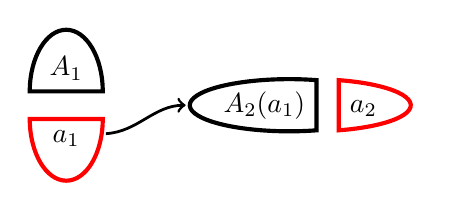
\begin{tikzpicture}
\tikzset{line width=1.5pt}
\node[name=a1,shape=swig hsplit, swig hsplit={line color lower=red}]{
        \nodepart{upper}{$A_1$}
        \nodepart{lower}{$a_1$}   };
\node[name=a2,shape=swig vsplit, right=of a1, swig vsplit={line color right=red}]{
         \nodepart{left}{$A_2(a_1)$}
         \nodepart{right}{$a_2$}  };
\draw[->,line width=1pt](a1) to[out=350,in=180] (a2);
\end{tikzpicture}

\end{center}

It has been hard to draw SWIGs using standard packages in TikZ/PGF.  Two separate {\tt semicircle} shapes can be used, but it is difficult to ensure that the two halves look as if they arise from a single circle, at least without introducing a lot of whitespace. TikZ does contain a shape, called {\tt split ellipse}, but this does not provide a way to add space between the two halves of the shape.
(There does not appear to be a semi-ellipse shape.)

We address this by introducing two multipart shapes: {\tt swig hsplit}  that creates an ellipse that has been split horizontally, and
and {\tt swig vsplit} that is split vertically. The latter shape also adjusts the ratio of the two halves depending on the text that is contained.

\eject
\subsection*{Preliminaries}

The examples included below use the following packages:
%%%%%
\begin{tkzltxexample}[]
\documentclass[10pt]{article}
\usepackage{amsmath,amssymb,xcolor}
\usepackage{pgf,tikz}
\usetikzlibrary{arrows,shapes.arrows,shapes.geometric,
shapes.multipart,decorations.pathmorphing,positioning,
swigs}
\begin{document}
...
\end{tkzltxexample}

%%%%%

%\noindent The last library listed here uses the code in the file:\par
%{\tt tikzlibraryshapes.swigs.code.tex} \par
%\noindent (As this is not part of the TeX distribution,  this file should be placed in the working directory.)




\subsection*{SWIG with horizontal split}

Here is a very simple example:

\begin{tkzexample}[very small,latex=4cm] 
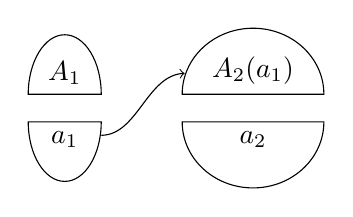
\begin{tikzpicture}
\node[name=a1,shape=swig hsplit]{
        \nodepart{upper}{$A_1$}
        \nodepart{lower}{$a_1$}   };
\node[name=a2,shape=swig hsplit,right=of a1]{
         \nodepart{upper}{$A_2(a_1)$}
         \nodepart{lower}{$a_2$}  };
\draw[->](a1) to[out=350,in=170] (a2);
\end{tikzpicture}
\end{tkzexample} 

\bigskip

\noindent The parameter {\tt gap} can be adjusted to change the size of the gap:



\begin{tkzexample}[latex=4cm, very small] 
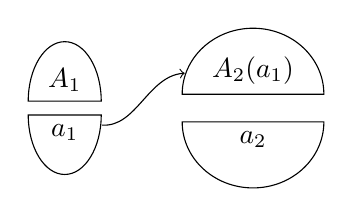
\begin{tikzpicture}
\node[name=a1,shape=swig hsplit,
swig hsplit={gap=5pt}]{
        \nodepart{upper}{$A_1$}
        \nodepart{lower}{$a_1$}  };
\node[name=a2,shape=swig hsplit, right=of a1]{
        \nodepart{upper}{$A_2(a_1)$}
        \nodepart{lower}{$a_2$}  };
\draw[->](a1) to[out=350,in=170] (a2);
\end{tikzpicture}
\end{tkzexample} 

\medskip
\eject

\noindent This can also be done globally for all split nodes;
here we also make the line color red for lower halves.

\begin{tkzexample}[latex=4cm, very small]
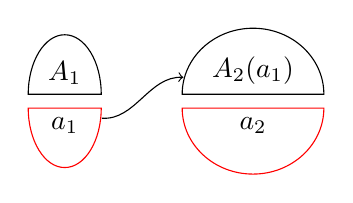
\begin{tikzpicture}
\tikzset{swig hsplit={gap=5pt,line color lower=red}}
\node[name=a1,shape=swig hsplit]{
        \nodepart{upper}{$A_1$}
        \nodepart{lower}{$a_1$} };
\node[name=a2,shape=swig hsplit, right=of a1]{
        \nodepart{upper}{$A_2(a_1)$}
        \nodepart{lower}{$a_2$} };
\draw[->](a1) to[out=350,in=170] (a2);
\end{tikzpicture}
\end{tkzexample}

\medskip

\noindent For black and white publications color may not be sufficient to distinguish
upper and lower halves. For this purpose a double line can be used.
{\tt inner line width lower} specifies the width of the inner gap.

\begin{tkzexample}[latex=4cm, very small]
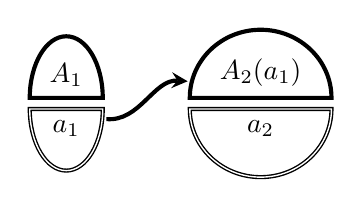
\begin{tikzpicture}
\tikzset{line width=1.5pt, 
    swig hsplit={gap=4pt,
                 inner line width lower=0.5pt}}]
\node[name=a1,shape=swig hsplit]{
        \nodepart{upper}{$A_1$}
        \nodepart{lower}{$a_1$} };
\node[name=a2,shape=swig hsplit, right=of a1]{
        \nodepart{upper}{$A_2(a_1)$}
        \nodepart{lower}{$a_2$} };
\draw[->,line width=1.5pt,>=stealth](a1) 
    to[out=350,in=170] (a2);
\end{tikzpicture}
\end{tkzexample}

\eject

\noindent The example below shows the full set of anchors and other options.

\begin{center}

\begin{tkzexample}[vbox, very small] 
\Huge
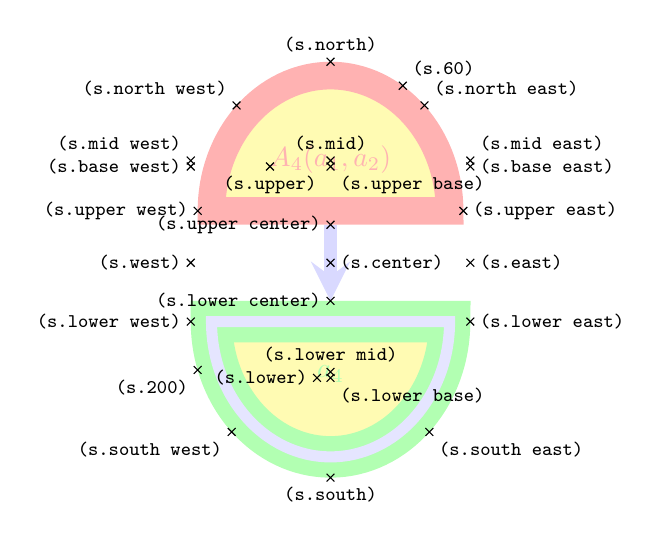
\begin{tikzpicture}
\pgfsetinnerstrokecolor{blue!10!white} % so inner line col=background
\tikzset{shape example/.style={fill=yellow!5,
            inner sep=0.3cm,outer sep=0cm}}
  \node[name=s, shape example, shape=swig hsplit,
       swig hsplit={
             line color upper=red!30, 
             fill color upper=yellow!30,
             line color lower=green!30,
             fill color lower=yellow!30,  
             gap=40pt,
             line width upper= 10pt, 
             inner line width upper = 0pt, 
             line width lower=15pt,  
             inner line width lower = 4pt}]
            {\nodepart[red!30]{upper}{$A_4(a_1,a_2)$}
             \nodepart[green!30]{lower}{$a_4$}};
  \draw[->,line width=5pt, draw=blue!15,>=stealth] 
                              (s.upper center) to (s.lower center);
  \foreach \anchor/\placement in
    {center/right, upper center/left, 
    upper/below, lower center/left, lower/left,
    60/above right,  200/below left, 
     mid/above, mid east/above right, mid west/above left,
     upper base/below right, base east/right, base west/left, 
     upper east/right, upper west/left,
     north/above, south/below, west/left, east/right,
     lower west/left, lower east/right,
     north east/above right, south east/below right, 
     south west/below left, north west/above left, 
     lower base/below right, lower mid/above}
     \draw[shift=(s.\anchor)] plot[mark=x] coordinates{(0,0)}
       node[\placement] {\scriptsize\texttt{(s.\anchor)}};   
\end{tikzpicture}
\end{tkzexample}
\end{center}

%%%%%%%%%%%%%%%%%%%%%%%%%%%%%%%%%%%%%%%%%%%%%%%%%%%%%

\eject

\subsection*{SWIG with vertical split}

Here we describe the instructions for creating ellipses with vertical splits. These are often more efficient in terms of space.
As before, first a very simple example:

\begin{tkzexample}[very small,latex=5.5cm] 
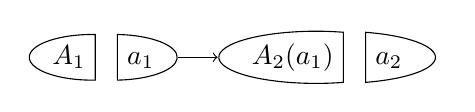
\begin{tikzpicture}
\node[name=a1,shape=swig vsplit]{
        \nodepart{left}{$A_1$}
        \nodepart{right}{$a_1$}  };
\node[name=a2, right=5mm of a1,
             shape=swig vsplit] {
             \nodepart{left}{$A_2(a_1)$}
             \nodepart{right}{$a_2$} };
\draw[->](a1) to (a2);
\end{tikzpicture}
\end{tkzexample} 

\bigskip

\noindent The parameter {\tt gap} can be adjusted to change the size of the gap:

\begin{tkzexample}[very small,latex=5cm] 
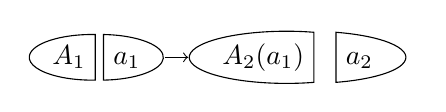
\begin{tikzpicture}
\node[name=a1,shape=swig vsplit,
  swig vsplit={gap=3pt}]{
        \nodepart{left}{$A_1$}
        \nodepart{right}{$a_1$}  };
\node[name=a2, right=3mm of a1,
             shape=swig vsplit] {
             \nodepart{left}{$A_2(a_1)$}
             \nodepart{right}{$a_2$} };
\draw[->](a1) to (a2);
\end{tikzpicture}
\end{tkzexample} 

\medskip

\noindent This can also be done globally for all split nodes;
here we also make the line color red for right halves.

\begin{tkzexample}[latex=5cm, very small]
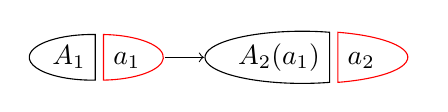
\begin{tikzpicture}
\tikzset{swig vsplit={gap=3pt,
                  line color right=red}}
\node[name=a1,shape=swig vsplit]{
        \nodepart{left}{$A_1$}
        \nodepart{right}{$a_1$} };
\node[name=a2,shape=swig vsplit, 
                  right=5mm of a1]{
        \nodepart{left}{$A_2(a_1)$}
        \nodepart{right}{$a_2$} };
\draw[->](a1) to (a2);
\end{tikzpicture}
\end{tkzexample}

\medskip

\eject

\noindent  As before, a version for black and white publications:

\begin{tkzexample}[latex=5cm, very small]
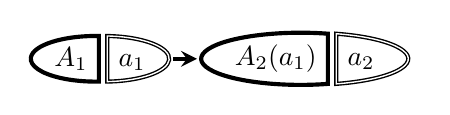
\begin{tikzpicture}
\tikzset{line width=1.5pt, 
         swig vsplit={gap=3pt,
         inner line width right=0.5pt}}
\node[name=a1,shape=swig vsplit]{
        \nodepart{left}{$A_1$}
        \nodepart{right}{$a_1$} };
\node[name=a2,shape=swig vsplit, 
                  right=3mm of a1]{
        \nodepart{left}{$A_2(a_1)$}
        \nodepart{right}{$a_2$} };
\draw[->,line width=1.5pt,>=stealth]
    (a1) to (a2);
\end{tikzpicture}
\end{tkzexample}

\bigskip

\noindent Here is an example with multiple stages:

\begin{tkzexample}[vbox]
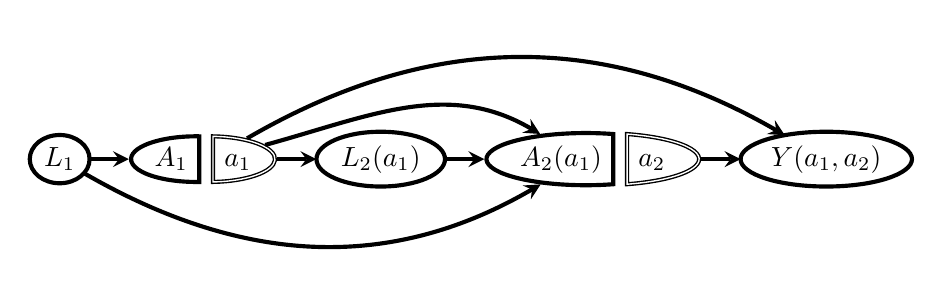
\begin{tikzpicture}
\tikzset{line width=1.5pt, outer sep=0pt,
         ell/.style={draw,fill=white, inner sep=2pt,
          line width=1.5pt},
         swig vsplit={gap=5pt,
         inner line width right=0.5pt}};
\node[name=l1, ell, shape=ellipse]{$L_1$};
\node[name=a1,right=5mm of l1, shape=swig vsplit]{
        \nodepart{left}{$A_1$}
        \nodepart{right}{$a_1$} };
\node[name=l2, right=5mm of a1, ell, shape=ellipse]{$L_2(a_1)$};
\node[name=a2,shape=swig vsplit, 
                  right=5mm of l2]{
        \nodepart{left}{$A_2(a_1)$}
        \nodepart{right}{$a_2$} };
\node[name=y, right=5mm of a2, ell, shape=ellipse]{$Y(a_1,a_2)$};
\draw[->,line width=1.5pt,>=stealth]
    (l1) edge (a1)
     (l1) edge[out=330,in=210] (a2)
    (a1) edge (l2)
    (a1) edge[out=15,in=150] (a2)
    (a1) edge[out=30,in=150] (y)
    (l2) edge (a2)
    (a2) edge (y);
\end{tikzpicture}
\end{tkzexample}





\eject

\noindent Expanded nodes showing additional options and anchors.

\begin{tkzexample}[vbox, very small] 
\Huge
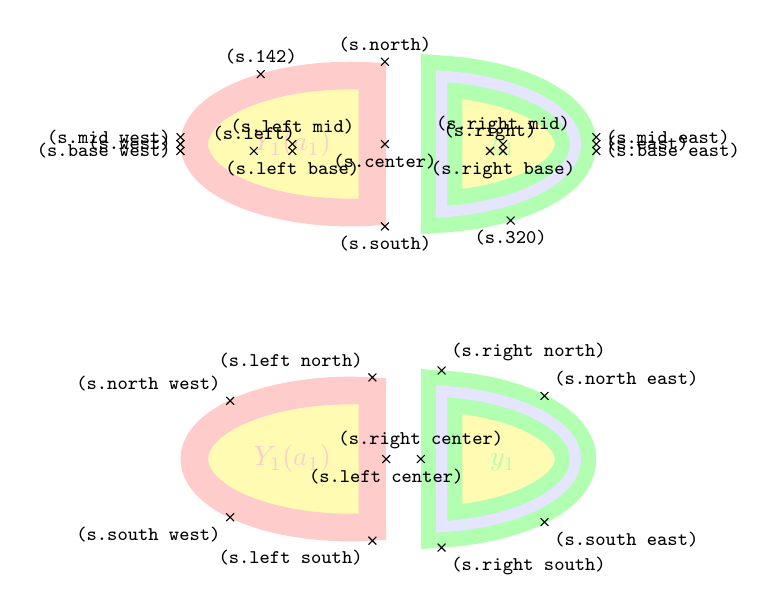
\begin{tikzpicture}
\pgfsetinnerstrokecolor{blue!10!white} % so inner line col=background
\tikzset{shape example/.style={draw,fill=yellow!30,
             inner xsep=10pt,inner ysep=25pt,outer xsep=0cm,outer ysep=0cm},
             swig vsplit={line color right=green!30, line color left=red!20, 
                        gap=25pt, line width left= 10pt, line width right=15pt,  
                      inner line width left = 0pt, inner line width right = 4pt}}
  \node[name=s,shape=swig vsplit, shape example]
            {\nodepart[red!20]{left}{$Y_1(a_1)$}
              \nodepart[green!30]{right}{$y_1$}};
 \foreach\anchor/\placement in 
  {north/above, south/below, east/right, west/left, 
 left base/below, right base/below, right/above, left/above,
 left mid/above, mid east/right, mid west/left, base east/right,
 base west/left, right mid/above,
 142/above, 320/below, center/below} 
  \draw[shift=(s.\anchor)] plot[mark=x] coordinates{(0,0)}
       node[\placement] {\scriptsize\texttt{(s.\anchor)}};
\begin{scope}[yshift=-4cm]
  \node[name=s,shape=swig vsplit, shape example]
  {\nodepart[red!20]{left}{$Y_1(a_1)$}%
 \nodepart[green!30]{right}{$y_1$}};
 \foreach\anchor/\placement in 
  {left center/below, right center/above, 
  left north/above left, left south/below left,
  right north/above right, right south/below right,
north west/above left, south west/below left,
 north east/above right, south east/below right} 
 \draw[shift=(s.\anchor)] plot[mark=x] coordinates{(0,0)}
       node[\placement] {\scriptsize\texttt{(s.\anchor)}};
 \end{scope}
 \end{tikzpicture}
\end{tkzexample}


\bibliographystyle{chicago}

\begin{thebibliography}{}

\bibitem[\protect\citeauthoryear{Richardson and Robins}{Richardson and
  Robins}{2013}]{swigs}
Richardson, T.S. and J.M.~Robins (2013).
\newblock Single world intervention graphs (SWIGs): A unification of
  counterfactual and graphical approaches to causality.
\newblock Working Paper Number 128. Available at
  \url{http://www.csss.washington.edu/Papers/wp128.pdf}.

\end{thebibliography}

%\bibliography{references}

\end{document}

